\section{Sistemas de control de versiones distribuidos} 
Es aquí donde entran los sistemas de control de versiones distribuidos (Distributed Version Control Systems o DVCSs en inglés). En un DVCS (como Git, Mercurial, Bazaar o Darcs), los clientes no sólo descargan la última instantánea de los archivos: replican completamente el repositorio. Así, si un servidor muere, y estos sistemas estaban colaborando a través de él, cualquiera de los repositorios de los clientes puede copiarse en el servidor para restaurarlo. Cada vez que se descarga una instantánea, en realidad se hace una copia de seguridad completa de todos los datos.

\begin{itemize}
	\begin{center}
	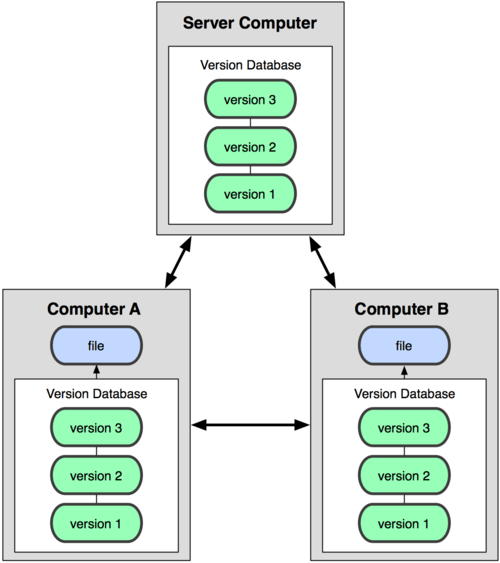
\includegraphics[width=14cm]{./Imagenes/imagen5} 
	\end{center}

	\item Es más, muchos de estos sistemas se las arreglan bastante bien teniendo varios repositorios con los que trabajar, por lo que puedes colaborar con distintos grupos de gente simultáneamente dentro del mismo proyecto. Esto te permite establecer varios flujos de trabajo que no son posibles en sistemas centralizados, como pueden ser los modelos jerárquicos.



\end{itemize} 